\documentclass[12pt, a4paper]{ctexart}
\usepackage{subcaption}
\usepackage{mystyle}
\usepackage{braket}
\usepackage{booktabs}
\newcommand{\bullshit}{bullshit}
\newcommand{\refbullshit}[1]{\ifdefined\bullshit #1\else\cite{empty}\fi}
\usepackage{physics}
\usepackage{graphicx}
\usepackage{lipsum}
% \usepackage{sectsty}
% \sectionfont{\fontsize{14}{\baselineskip}\selectfont}
% \subsectionfont{\fontsize{12}{\baselineskip}\selectfont}
\usepackage[hypertexnames=true]{hyperref}
\usepackage{cleveref}
\usepackage{siunitx}
\usepackage{geometry}
\geometry{
  paper      = a4paper,
  vmargin    = 2.54cm,
  hmargin    = 3.17cm,
  headheight = 0.75cm,
  headsep    = 0.29cm,
  footskip   = 0.79cm,
}
\usepackage{authblk}
\usepackage{lmodern}
\makeatletter
\renewenvironment{abstract}{%
    \if@twocolumn
      \section*{\abstractname}%
    \else %% <- here I've removed \small
      \begin{center}%
        {\bfseries \large\abstractname\vspace{\z@}}%  %% <- here I've added \Large
      \end{center}%
      \quotation
    \fi}
    {\if@twocolumn\else\endquotation\fi}
\makeatother
\usepackage{zhlipsum}
% \usepackage[section]{placeins}
% \newcommand\blankpage{%
%     \null
%     \thispagestyle{empty}%
%     \addtocounter{page}{-1}%
%     \newpage}
\usepackage{mystyle}
\usepackage{afterpage}
\usepackage[ruled,vlined]{algorithm2e}
\SetAlgorithmName{算法}{算法}{算法清单} 
\usepackage{longtable}
\usepackage{siunitx}
\usepackage{subcaption}
\usepackage{cleveref}
\makeatletter

\newdimen\bp@
\bp@=1bp
\crefname{equation}{式.}{式.}
\crefname{figure}{图.}{图.}
% \renewcommand{\refname}{\centerline{参考文献及注释}}
\begin{document}
\begin{titlepage}%
    \centering
    
\includegraphics[height=0.8cm]{figures/ustc-name.pdf}\par
    {\sffamily\fontsize{20\bp@}{20\bp@}\selectfont
      大学生研究计划结题报告\par}%
      % \vspace{-1.5cm}
    \parbox[t][1.5cm][c]{\textwidth}{%
      \centering\sffamily\bfseries\fontsize{15\bp@}{15\bp@}\selectfont
      高能核物理实验中B介子横动量谱及核修正因子的研究\par}
     % \vspace{-1.5cm}
      \parbox[t][3cm][t]{\textwidth}{%
      \centering\sffamily\bfseries\fontsize{12\bp@}{12\bp@}\selectfont
      Study of B meson transverse momentum spectrum and its nuclear modification factors in high energy nuclear physics experiment.\par\par}

    {\fontsize{12\bp@}{12\bp@}\selectfont
      \begin{tabular}{ll}%
        \textsf{作者姓名:} & 周鹏宇 \\
        \textsf{学号:} & PB18000165\\
        \textsf{院系:} & 少年班学院~~近代物理系\\
        % \textsf{\ustc@speciality@name:} & \ustc@speciality \\
          \textsf{导师姓名:} & 张一飞~~教授 \\
          \textsf{日期:} & 二〇二一年三月 \\
        % \textsf{完成时间:} & \date{today}\\
      \end{tabular}\par}%
\begin{abstract}
研究夸克解禁闭的新物质相——夸克胶子等离子体(QGP),是高能核物理领域最前沿最重要的根本科学问题。底夸克被认为是研究QGP理想的探针。但是在实验上,只能探测B介子衰变子粒子的动量谱。我们从已有的实验数据中分析,通过衰变产物产生谱及底强子的衰变运动学,首次提取了底强子的横动量谱。通过上述横动量谱计算了相关的核修正因子($R_{AA}$),在误差范围内与RHIC-STAR观测的实验数据一致。

\end{abstract}

\renewcommand{\abstractname}{Abstract}

\begin{abstract}
	The properties of the quark-gluon plasma(QGP) is an unsolved problem in physics. Formed in the initial collision, the bottom quark is regarded as the ideal probe of the QGP. However, in real experiments, only the decayed daughter particles of B meson can be detected. We present the work of obtaining the transverse momentum spectrum of B meson using a data-driven method. Moreover, we used such spectrum to calculate the relevant nuclear modification factor($R_{AA}$). Compared to the results observed in RHIC-STAR, these results are within error range.
\end{abstract}
\end{titlepage}%

\tableofcontents

\section{简介} % (fold)
\label{sec:简介}

\subsection{研究背景} % (fold)
\label{sub:物理背景}

高重子数密度或者高温是产生QGP的条件。后者在高能重离子碰撞实验中可以实现。重味夸克在高能重离子碰撞的初期产生,它可以经历QGP的整个演化过程,因此重味(底夸克)被认为是研究QGP理想的探针。除此以外,因为底夸克质量远大于轻夸克和QCD能标,可由微扰QCD精确计算,测量底夸克产生谱和截面对检验QCD理论有重要的科学意义。\par
另一方面,底夸克在热核介质中与介质相互作用目前尚不清楚,理论预言底夸克能损在QGP中相较于其它轻夸克和粲夸克要小,这种质量效应在底夸克衰变产物的测量中被发现,但是STAR的数据在不同的衰变道中子粒子核修正因子($R_{AA}$)似乎有「不一致」的情况。\cite{SI2020135465}但是,目前为止,还未有对底强子的直接测量,原因是底夸克产生截面极低,强子道衰变分支比都在千分之一甚至更低,因此要实现底强子产生谱与底夸克产生截面的测量具有极大的挑战性。
\par
本课题的目的主要解决两个问题:1)检验STAR数据在不同衰变道的结果的一致性;2)实现底强子产生谱和产生截面的首次测量。\par
% subsection 物理背景 (end)

\subsection{研究思路} % (fold)
\label{sub:研究思路}
我们用B介子代表底夸克。我们得到B介子产生谱(横动量谱$\eddon{^2N}{p_T\rd y}$)的主要思路是,以猜测的L\'evy函数分布进行抽样,通过对B介子衰变运动学的Monte Carlo模拟来得到其衰变子粒子的横动量谱$\frac{\rd^2N}{2\pi p_T\rd p_T\rd y}$,将该数据与实验进行比较,计算描述误差的统计量并通过算法减小误差。此时,问题转换为无约束最优化问题,该问题可以用模拟退火法解决。优化参数后,给出拟合结果的同时我们就得到了B介子的产生截面。\par
接下来,我们将得到拟合结果结合FONLL\cite{cacciari2012theoretical}的数据用于计算核修正因子($R_{AA}$),与实验数据\cite{Tang:2020ame}比较,证实在误差范围内,同一种B粒子的分布也会导致不同衰变道$R_{AA}$的不一致,最终得到结论。

% subsection 研究思路 (end)

% section 简介 (end)

\section{B介子谱的确定} % (fold)
\label{sec:b粒子谱的确定}
我们需要确定AuAu碰撞下B介子的横动量谱。现有的数据是$\sqrt{s_{NN}}=\SI{200}{\GeV}$,RHIC观测到的b$\to$e的谱$\frac{\rd^2N}{2\pi p_T\rd p_T}$\cite{SI2020135465},我们用这个谱作为数据来拟合母粒子的谱。
\subsection{抽样} % (fold)
\label{sub:抽样}
我们以B$^0$介子来模拟b的衰变。由统计力学的分析\cite{tsallis1999nonextensive},可以用L\'evy-Tsallis函数来拟合B介子的横动量分布$\eddon{^2N}{p_T\rd y}$,其具体形式为
\begin{equation}\label{levy}
\eddon{^2N}{p_T\rd y} \equiv f(p_T) = \eddon{N}{y}\frac{(n-1)(n-2)}{2\pi n C\brac{nC+m_0(n-2)}}\times\pare{1+\frac{\sqrt{p_T^2+m_0^2}-m_0}{nC}}^{-n}	
\end{equation}
其中$\rd y$取为2,表示$B$粒子的快度区间长度,$n,C,\eddon{N}{y}$是未知自由参数,$m_0$表示B介子的静止质量(\si{\GeV\per c^2})。抽样时,指定B$^0$介子的各个参数。为了提高抽样效率,令其$p_T$均匀分布而在填充直方图时,选取权重为Levy函数在相应$p_T$的值,表示实际对应的粒子数(\cref{weight})。
\begin{equation}\label{weight}
	p_T\sim U[0,20),\quad \text{\texttt{weight}}=f(p_T)
\end{equation}
在实际模拟时,需按照\cref{p,y,e}指定\cite{explaination}母粒子(B$^0$粒子)动量$p_x,p_y,p_z$,能量$E$。
\begin{equation}
\label{p}
	\varphi\sim U[0,2\pi],\quad p_x = p_T\sin\varphi,\,
			p_y = p_T\cos\varphi \end{equation}\begin{equation}
		\label{y}
	y\sim N(0, 1.2)\quad p_z = \sqrt{m^2+p_T^2}\sinh y\end{equation}\begin{equation}
	\label{e}
	P = \sqrt{p_T^2+p_z^2} \quad E = \sqrt{P^2+m^2} 
\end{equation}

% subsection 抽样 (end)

\subsection{Monte Carlo模拟} % (fold)
\label{sub:monte_carlo模拟}

我们使用\texttt{PYTHIA8}\cite{Sj_strand_2015}来模拟B$^0$粒子衰变的动力学过程。对每次抽样,仅仅打开B$^0\to$e$+$X(X是任意其他粒子)的衰变道,提取子粒子的横动量填充直方图$\frac{\rd^2N}{2\pi p_T\rd p_T\rd y}$。其中,为保持与实验一致,筛选$\abs{y}<0.7$的e进行填充。

在抽样完成后,直方图需归一化,归一化系数为
\begin{equation}
	\frac{BR\times N}{\sum\text{\texttt{weight}}} = \frac{BR\times\int_{-1}^1\rd y\int_0^{20}\rd p_T\frac{\rd^2N}{\rd p_T\rd y}}{\sum\text{\texttt{weight}}}
\end{equation}
其中$\sum\text{\texttt{weight}}$表示参与抽样的粒子数,$BR$是分支比(选用\texttt{PYTHIA8}的数据,为\num{0.1061984}),$N$是在实验中B介子的产量。

在实际抽样过程中,为提高抽样速度,采取并行算法,用\texttt{HTCondor}同时运行100个程序产生100个直方图,最后对直方图进行合并得到模拟结果。


% subsection monte_carlo模拟 (end)

\subsection{无约束最优化问题} % (fold)
\label{sub:无约束最优化问题}

通过L\'evy函数(\cref{levy})的三个参数(记为$\+vp$),定义统计量
\begin{equation}
x^2(\+vp)=\sum_{n=1}^N\frac{(f_\text{cal}-f_\text{exp})}{\sigma^2}\sim\chi^2(N-1) 
\end{equation}
其中$f_\text{cal}$是\nameref{sub:monte_carlo模拟}得到的电子谱,$f_\text{exp}$是实验上测得的电子谱,$\sigma^2$是统计误差,$N$是采用的数据点个数。\par
采用模拟退火法寻找其极小值,算法如下:\par
\begin{algorithm}[htb]
  \small
  % \SetAlgoLined
  % \KwData{this text}
  \KwResult{参数$\+vp$及其对应的$x^2(\+vp)$ }

  设定步长$\+v\varepsilon=(\num{2e-4}, \num{0.002}, \num{0.05})$,设定温度与步数$i$的函数$T=0.95^{-i}$\;
  \While{步数$<$设定最大步数}{
    计算$x^2(\+vp)$\;
   	产生一个随机向量$\+v\xi\sim U[-1,1]^3$。计算$x^2(\+vp+\+v\xi\times\varepsilon)$,这里乘法是逐项相乘 \;
   	产生随机数$\xi\sim U[0,1)$\;
    \If{$\xi<\min\pare{1,\exp(-(x^2-x'^2)/T)}$}{
      $\+vp=\+vp+\+v\xi$\;
  }
  }
  \caption{模拟退火法}
  \label{algo:algorithm1}
\end{algorithm}
目前结果是
\begin{equation}\label{params}
	\frac{\rd N}{\rd y} = \num{1.50e-02},\,C = \num{0.276},\,n = \num{5.40},\, x^2=\num{19.897402}
\end{equation}
我们使用的数据点是19个,根据$\chi^2$检验方法
\begin{equation}
	CDF(\chi^2(18),\num{19.897402})=\num{0.66138}
\end{equation}
在$P=\num{0.34}$内不能否定原假设。\par
模拟结果如\cref{b2e}所示,在误差范围内,Monte Carlo模拟结果和实验结果相符。
\begin{figure}[h]\centering
	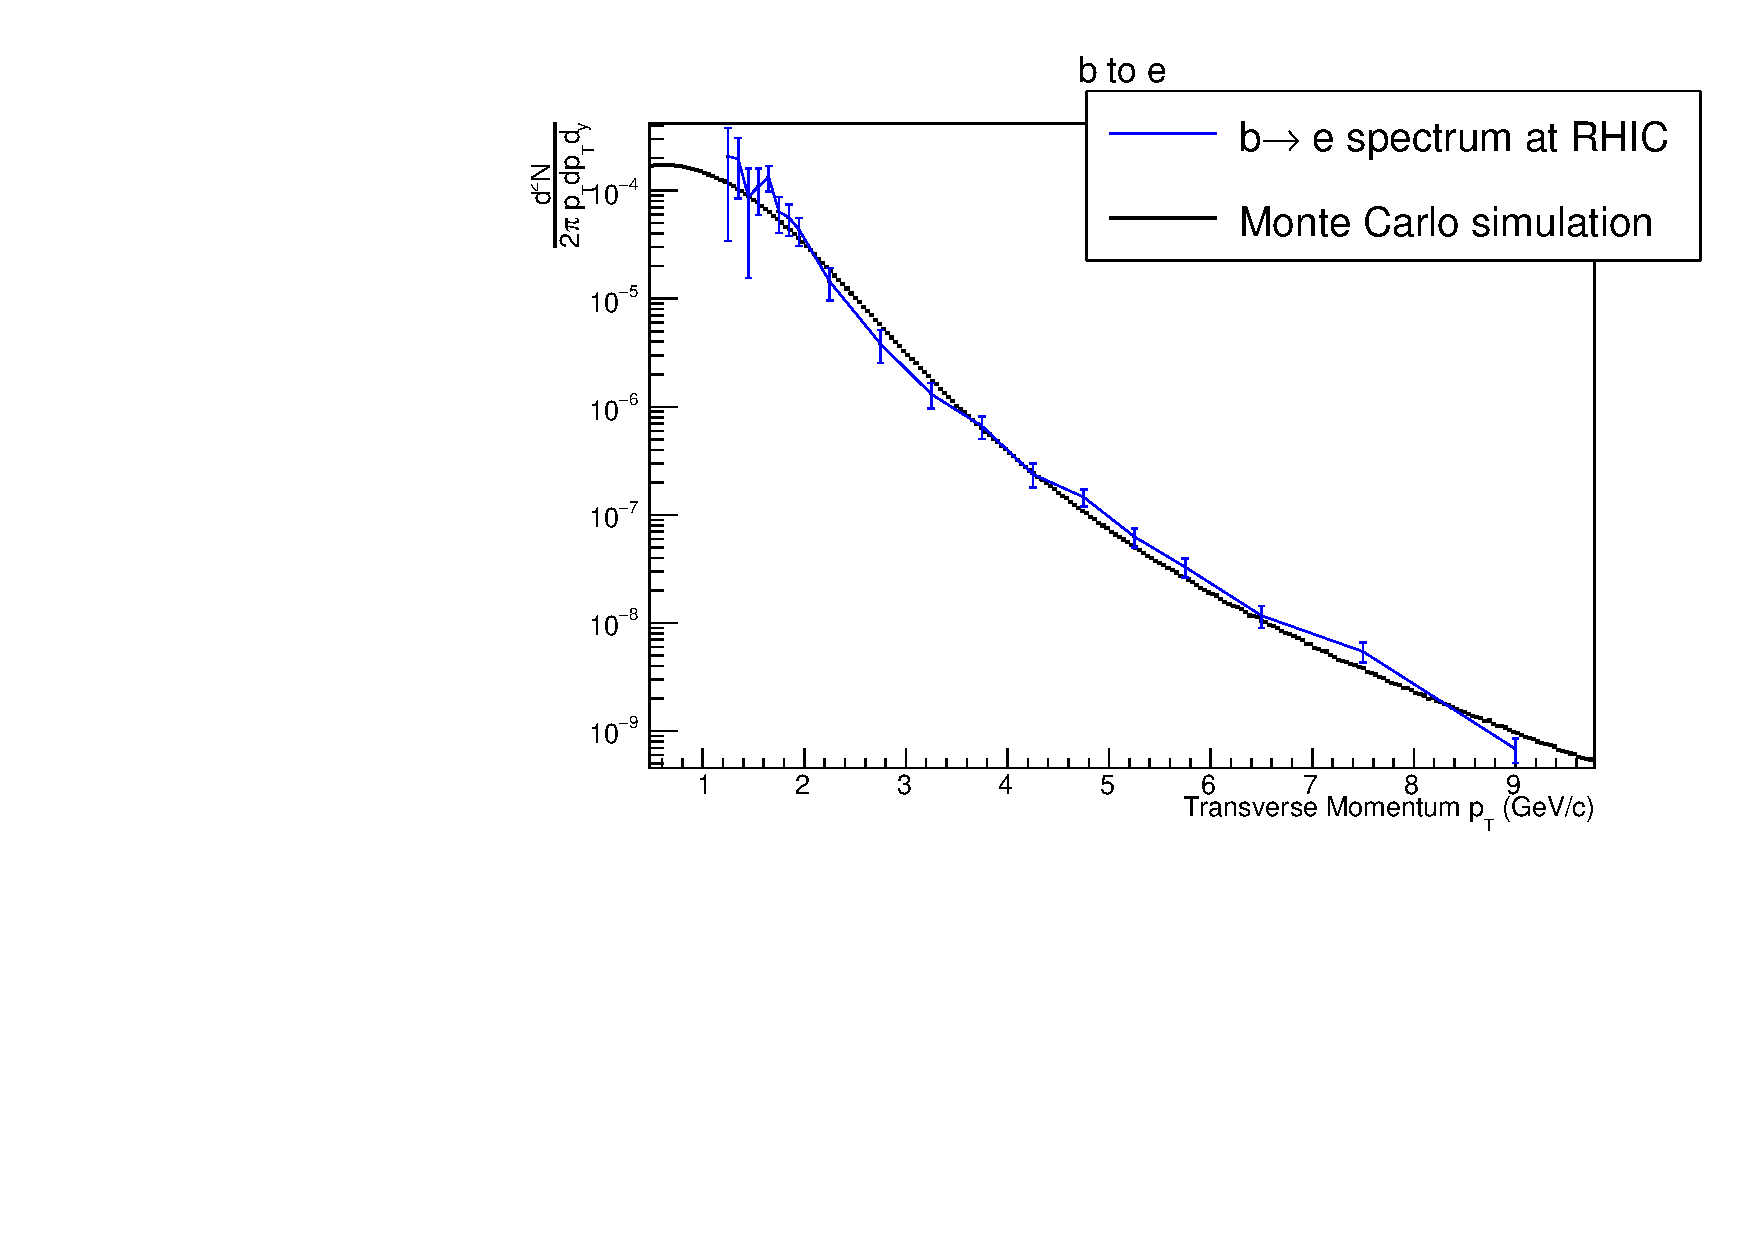
\includegraphics[width=8cm]{figures/unnamed.pdf}
	\caption{b$\to$e RHIC测量的结果和Monte Carlo模拟结果的比较}
	\label{b2e}
\end{figure}
% subsection 无约束最优化问题 (end)

\subsection{结论} % (fold)
\label{sub:结论}

通过\texttt{PYTHIA8}\cite{Sj_strand_2015}的Monte Carlo模拟和模拟退火算法,可以定下用于拟合B介子横动量谱的L\'evy函数的三个参数,并在误差范围内和实验数据相符。
\par 通过\cref{params}定下的参数,我们可以算出底夸克的产生截面。单位快度内,从产量$\eddon{N}{y}$换算为截面$\eddon{\sigma}{y}$的公式为
\begin{equation}
	\eddon{\sigma}{y} = \eddon{N}{y}\times\eddon{\sigma^{pp}_{\text{inel}}}{N_\text{bin}} = \SI{2.16}{\micro\barn}
\end{equation}
其中$\sigma^{pp}_{\text{inel}}=\SI{42}{\milli\barn}$表示pp碰撞截面,$N_\text{bin}=\num{291.90194}$表示平均二夸克碰撞的次数\cite{Zhang:2008gb}。
\par 但是观察\cref{b2e}发现,RHIC的$p_T$谱测量结果在较低横动量有很大的误差,甚至存在较大波动。我们认为,测量误差是导致算出的$\chi^2$最小也有19,拟合不会达到更优的主要原因。

% subsection 结论 (end)


% section b粒子谱的确定 (end)

\section{核修正因子} % (fold)
\label{sec:核修正因子}

核修正因子定义为重离子碰撞的产额除以质子碰撞的产额后,用碰撞数归一化后得到的结果
\begin{equation}\label{raa}
	R_{AA} = \frac{\rd^2N_{AA}/2\pi p_T\rd p_T\rd y}{N_\text{bin}\rd^2N_{pp}/2\pi p_T\rd p_T\rd y} = \frac{\rd N_{AA}/\rd p_T}{N_\text{bin}\rd N_{pp}/\rd p_T}
\end{equation}
其中$N_\text{bin}$为核子-核子碰撞数,取为\num{291.90194}。$R_\text{AA}$与1的偏离用于表示粒子在高能核碰撞中与QGP作用的能量变化情况。\par
在实验上,已获取了测得B介子衰变到e,D$^0$,J/$\psi$子粒子的$R_{AA}$,我们用上一节确定的母粒子谱的数据抽样分子,计算子粒子的$R_{AA}$并与实验数据比较。

\subsection{分母的分布} % (fold)
\label{sub:分母的分布}
需要用pp碰撞产生的B介子分布抽样分母。
\texttt{FONLL}模型\cite{cacciari2012theoretical}已经计算了分母的分布,我们使用该模型的数据,用Levy函数拟合,结果为
\begin{equation}\label{sigma}
	\frac{\rd N}{\rd y} = \num{1.804e-05}\quad C = \num{0.6897}\quad N = \num{10.00}
\end{equation}
\par
然而,我们在调研文献中发现,\texttt{FONLL}模型与实验测量值\cite{Aidala:2019hib}相差较大。因此,我们采用与上一节同样的算法,找到pp碰撞中b$\to$e的e的谱\footnote{我们使用的数据是b$\to$e的截面$\rd\sigma$的谱,产量$\rd N$谱需要乘以30转化为截面(利用\cref{sigma})。},拟合得到B介子分布的Levy函数的三个参数为
\begin{equation}
	\frac{\rd N}{\rd y} = \num{3.616e-05}\quad C = \num{0.6696}\quad N = \num{9.740}\quad x^2=\num{1.30434e-01} 
\end{equation}
我们使用了21组数据
\begin{equation}
	CDF(\chi^2(20),\num{1.30434e-01})\approx\num{4e-19}
\end{equation}
因此,在$P=1.000$内不能否定原假设(\cref{b2ep})。
\begin{figure}[h]\centering
	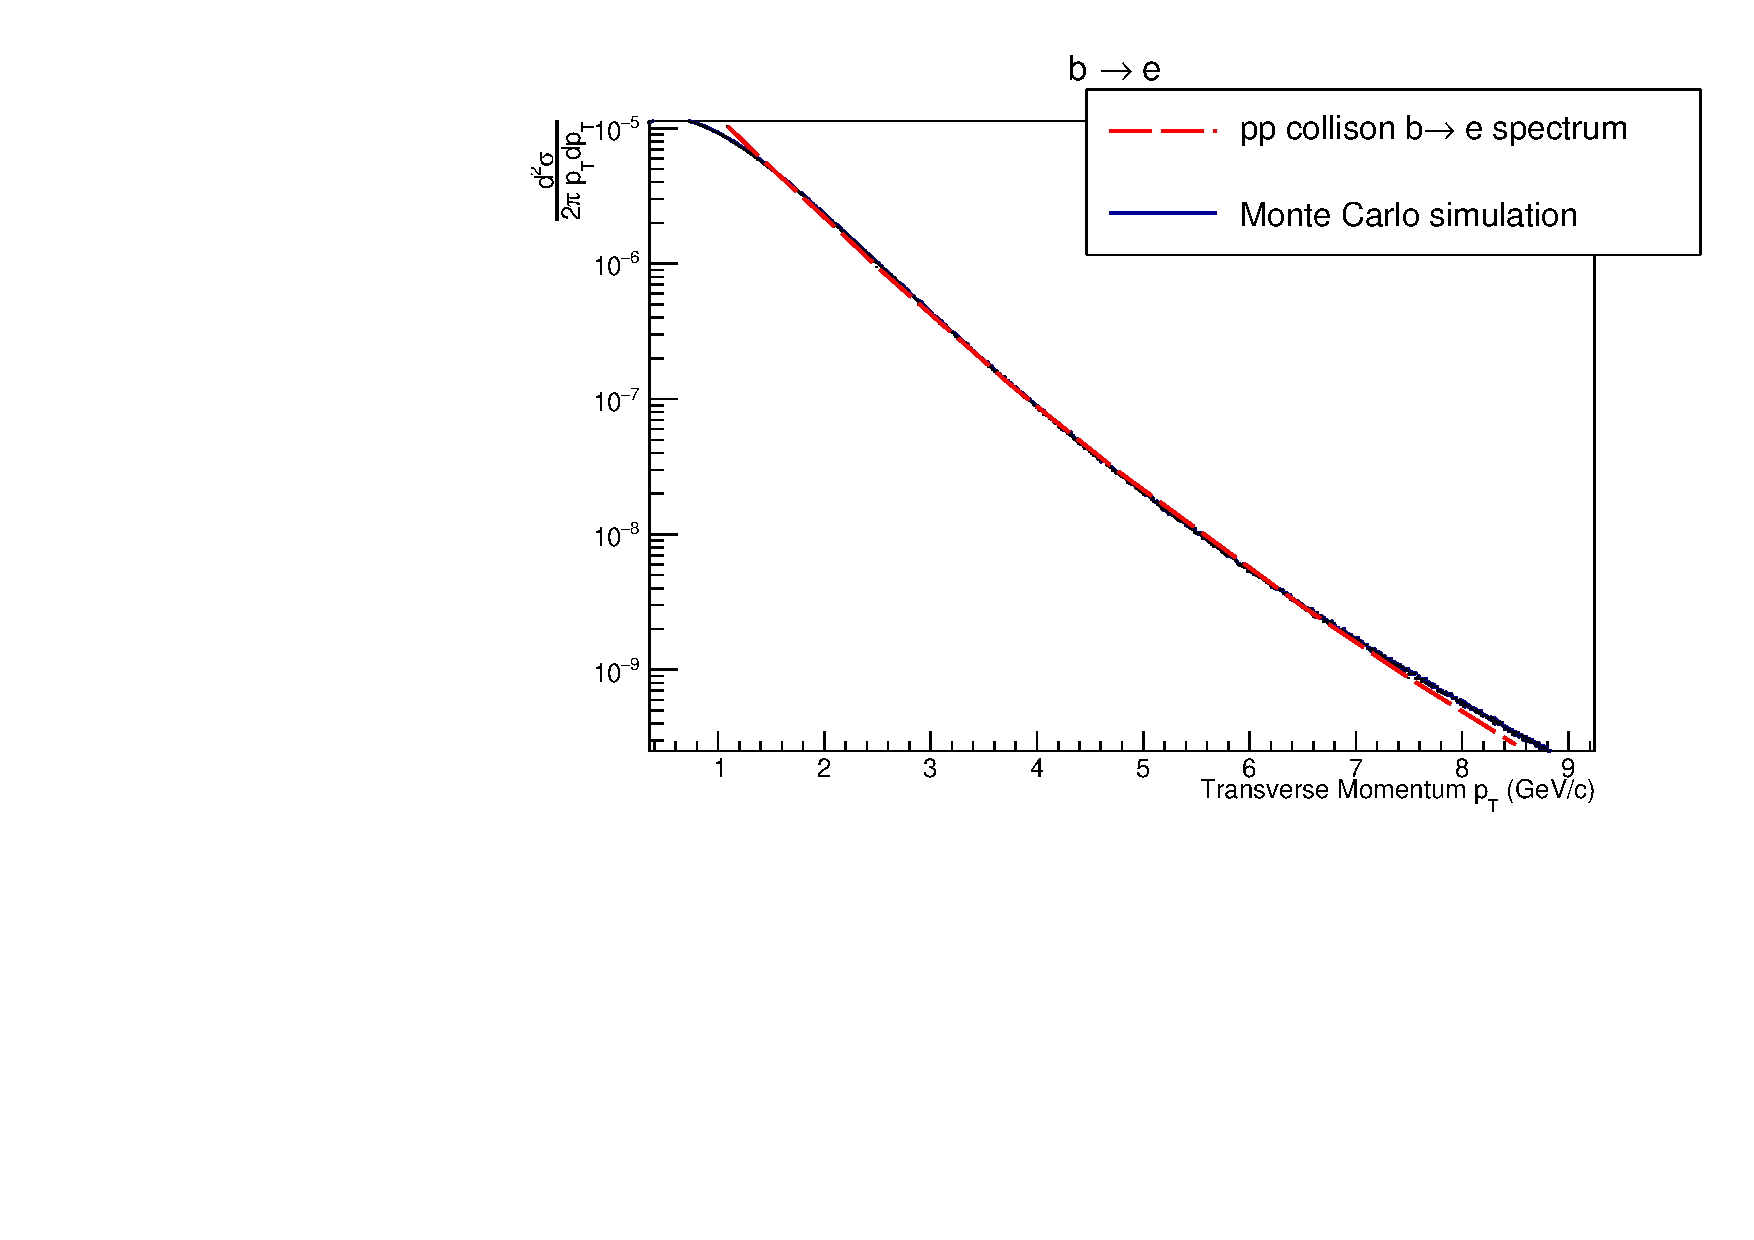
\includegraphics[width=8cm]{figures/pp.pdf}
	\caption{pp碰撞 b$\to$e 测量的结果和Monte Carlo模拟结果的比较}
	\label{b2ep}
\end{figure}
但是,考虑到实验测量上仍存在一定误差,我们保留这两种参数用于计算$R_{AA}$。
% subsection 分母的分布 (end)

\subsection{计算} % (fold)
\label{sub:计算}
按照\cref{raa},计算步骤为
\begin{algorithm}[htb]
  \small
  \For{子粒子\textnormal{\textbf{in}} e,D$^0$,J/$\psi$}{
   打开子粒子衰变道\;
   初始化分母$B^0$粒子分布(按分子Levy函数参数初始化)\;
   Monte Carlo模拟AA碰撞子粒子的$p_T$直方图\;
   初始化分子$B^0$粒子分布(按分母Levy函数参数初始化)\;
   Monte Carlo模拟pp碰撞子粒子的$p_T$直方图\;
   两个直方图分别归一化\;
   直方图相除,绘制$R_{AA}$\;
  }
  \caption{计算$R_{AA}$}
  \label{algo:algorithm1}
\end{algorithm}

% subsection 计算 (end)

\subsection{结论} % (fold)
\label{sub:结论}


\begin{figure}[h]
\begin{subfigure}[h]{0.5\textwidth}\centering
	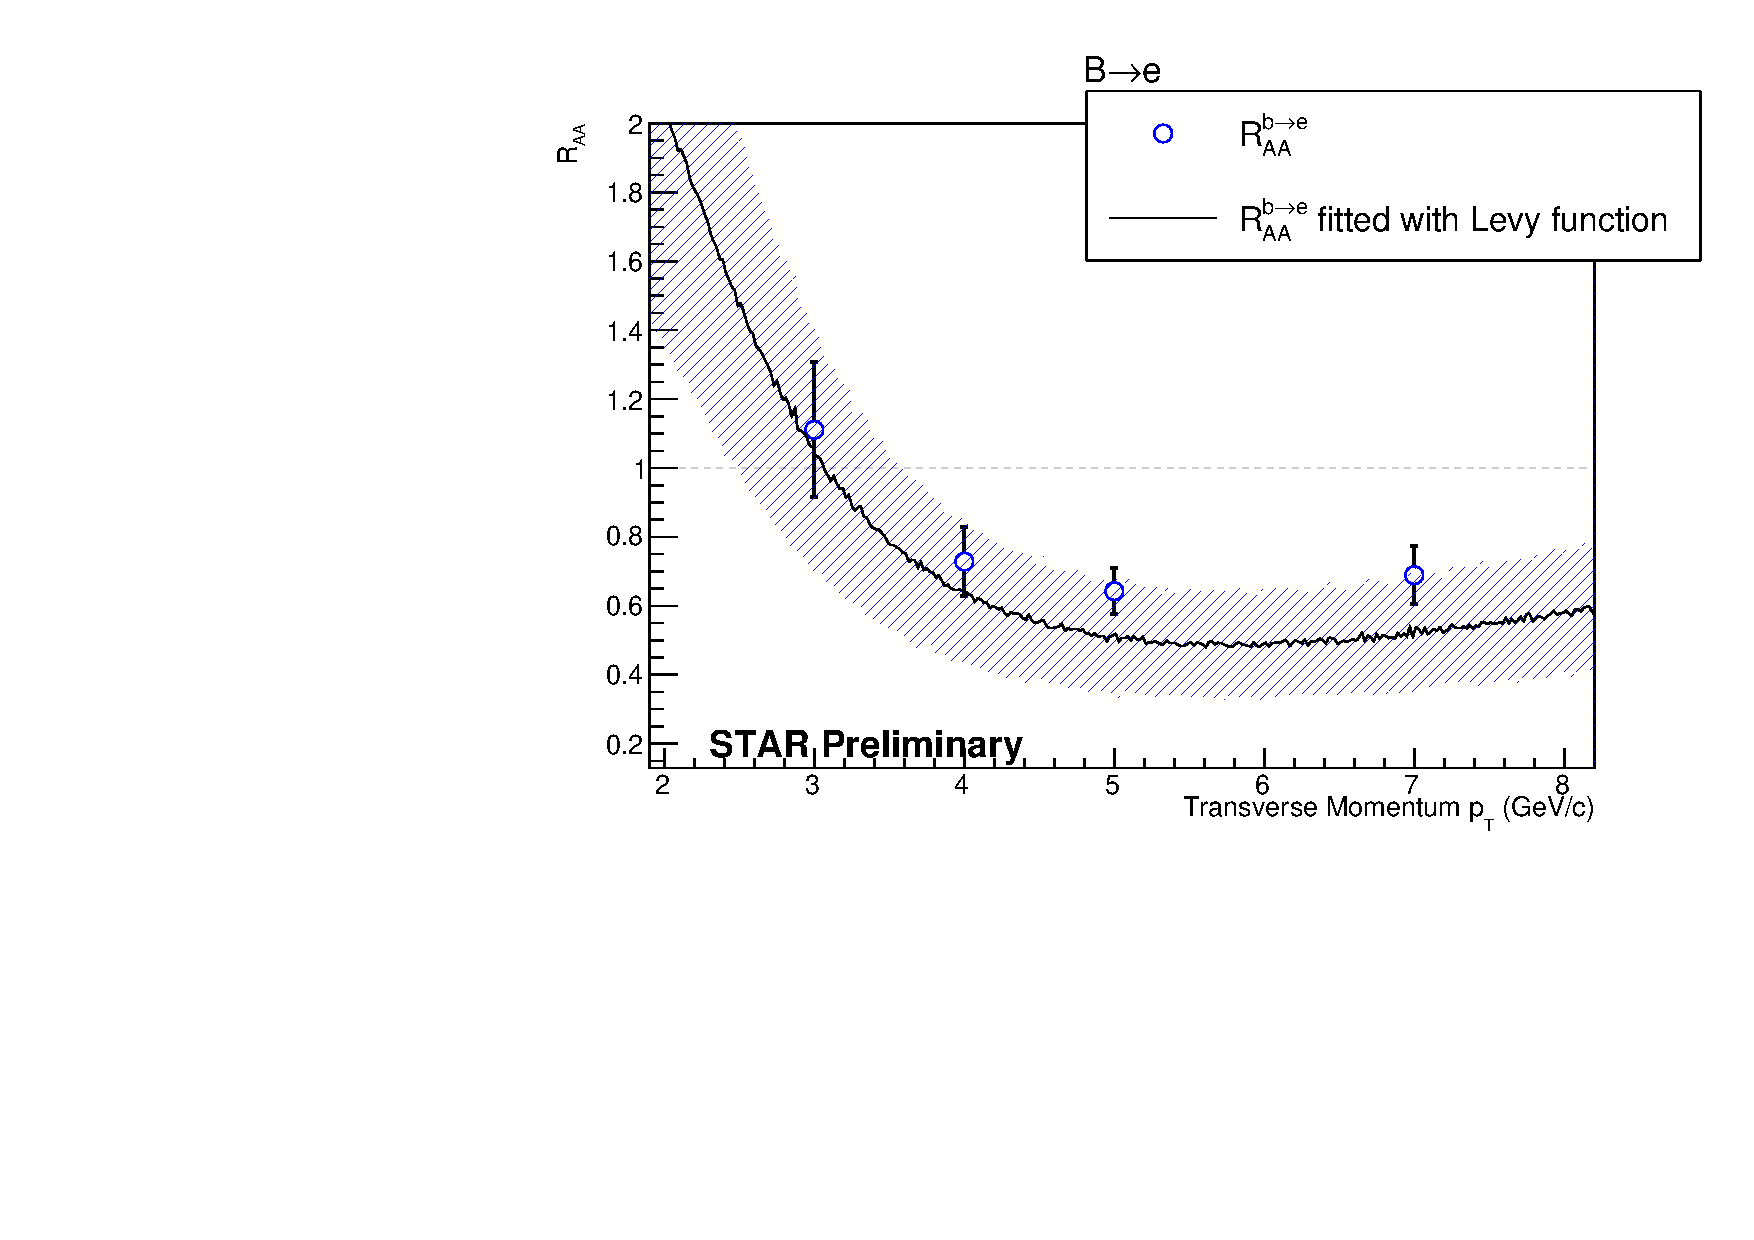
\includegraphics[width=7.5cm]{figures/B2e.pdf}
	\caption{b$\to$e $R_{AA}$}
	\label{b2e0}
\end{subfigure}
\begin{subfigure}[h]{0.5\textwidth}\centering
	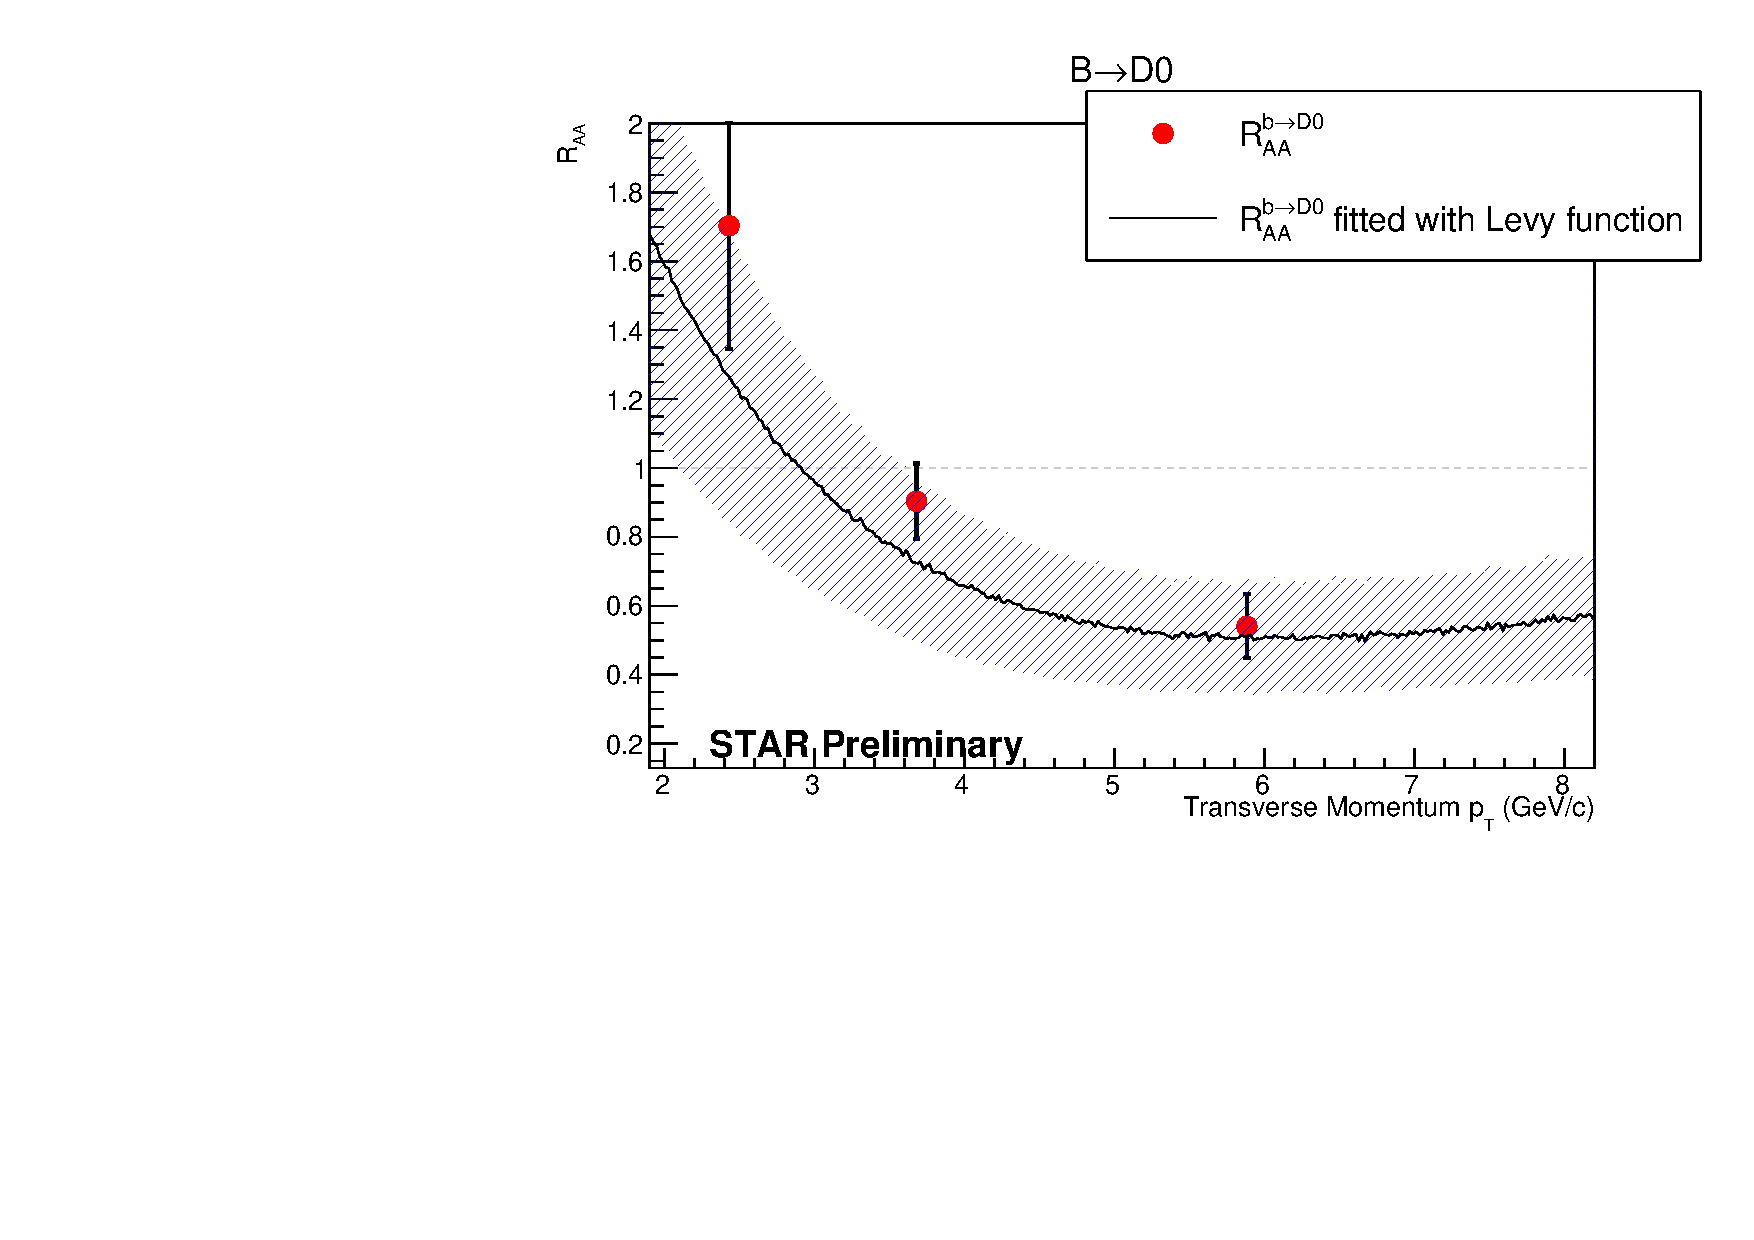
\includegraphics[width=7.5cm]{figures/B2D0.pdf}
	\caption{b$\to$D$^0$ $R_{AA}$}
	\label{b2d}
\end{subfigure}
\caption{$R_{AA}$的计算结果}
\end{figure}
\begin{figure}[h]
	\begin{subfigure}[h]{0.5\textwidth}\centering
	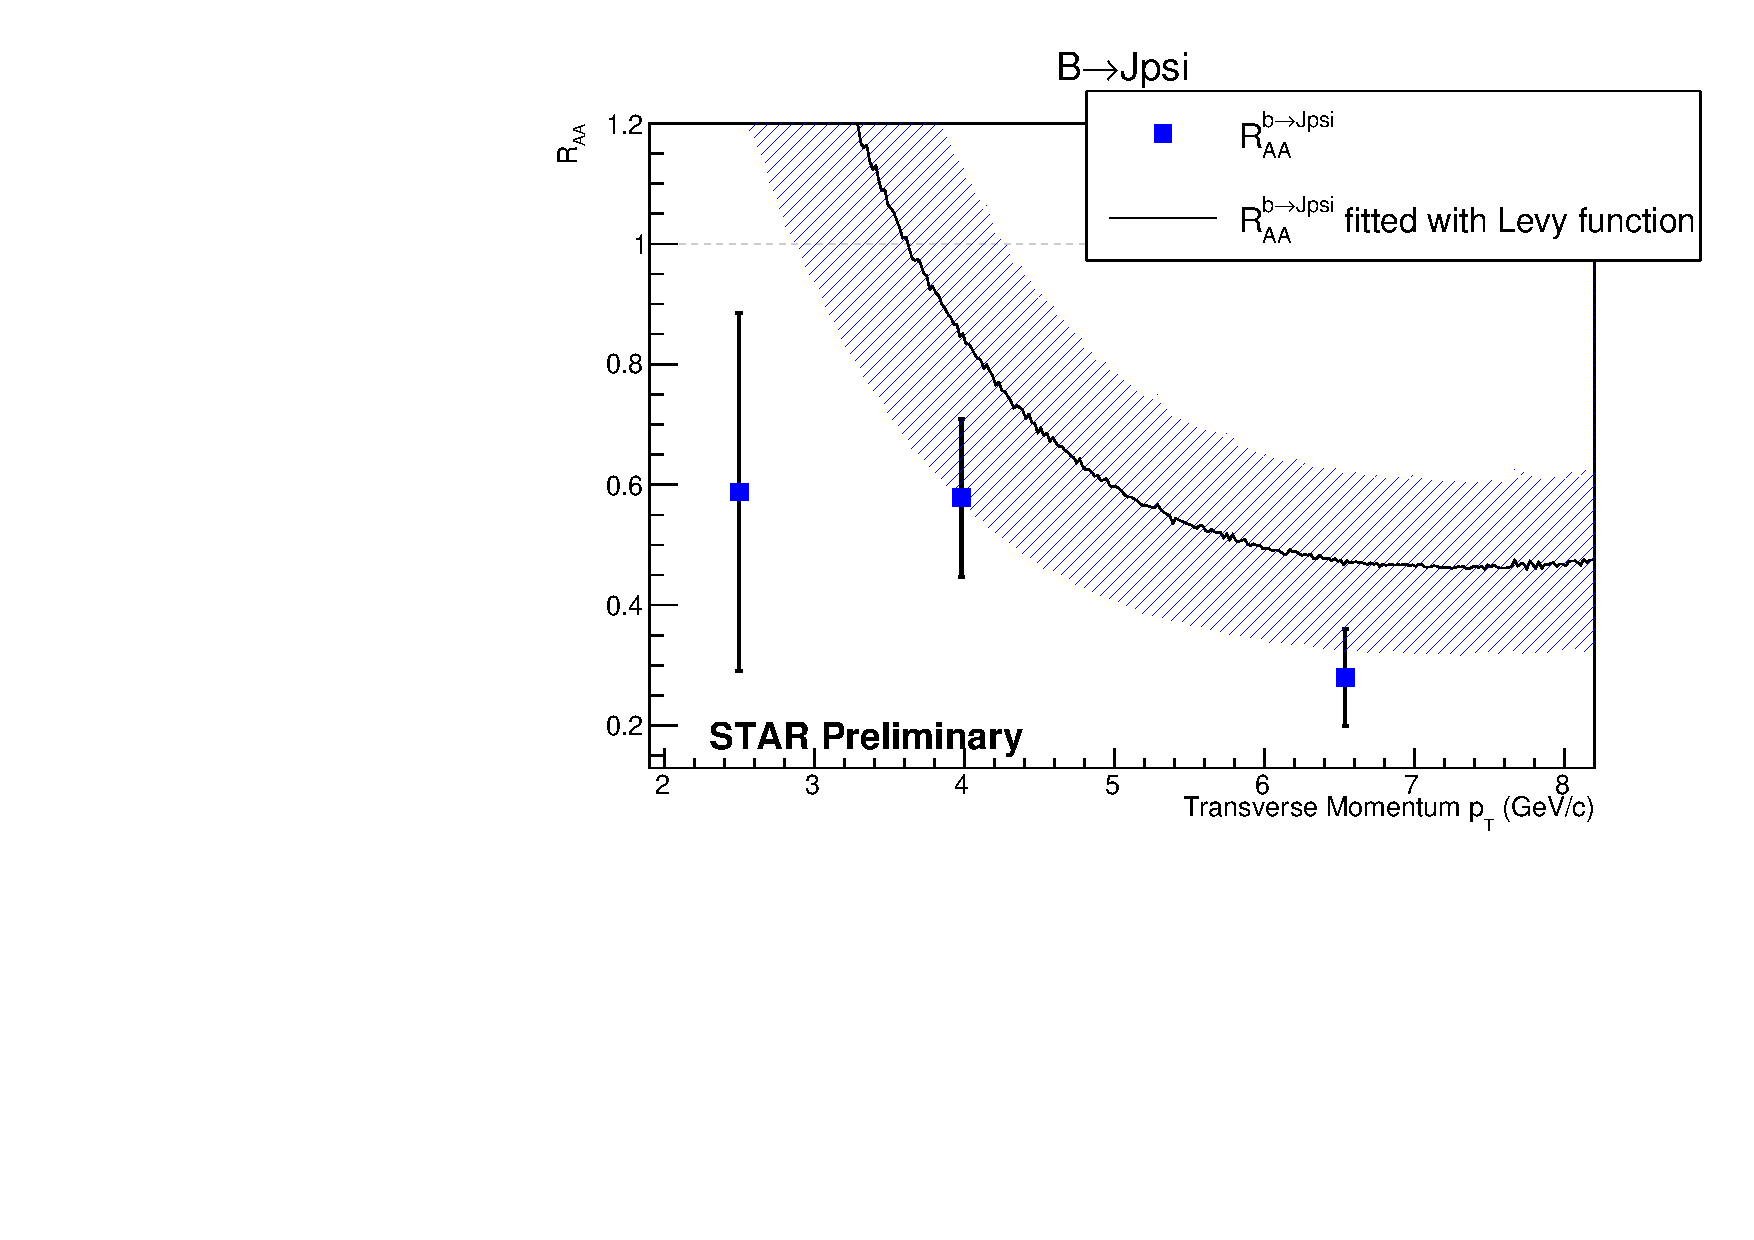
\includegraphics[width=7.5cm]{figures/B2Jpsi.pdf}
	\caption{b$\to$J/$\psi$ $R_{AA}$}
	\label{b2j}
\end{subfigure}
\begin{subfigure}[h]{0.5\textwidth}\centering
	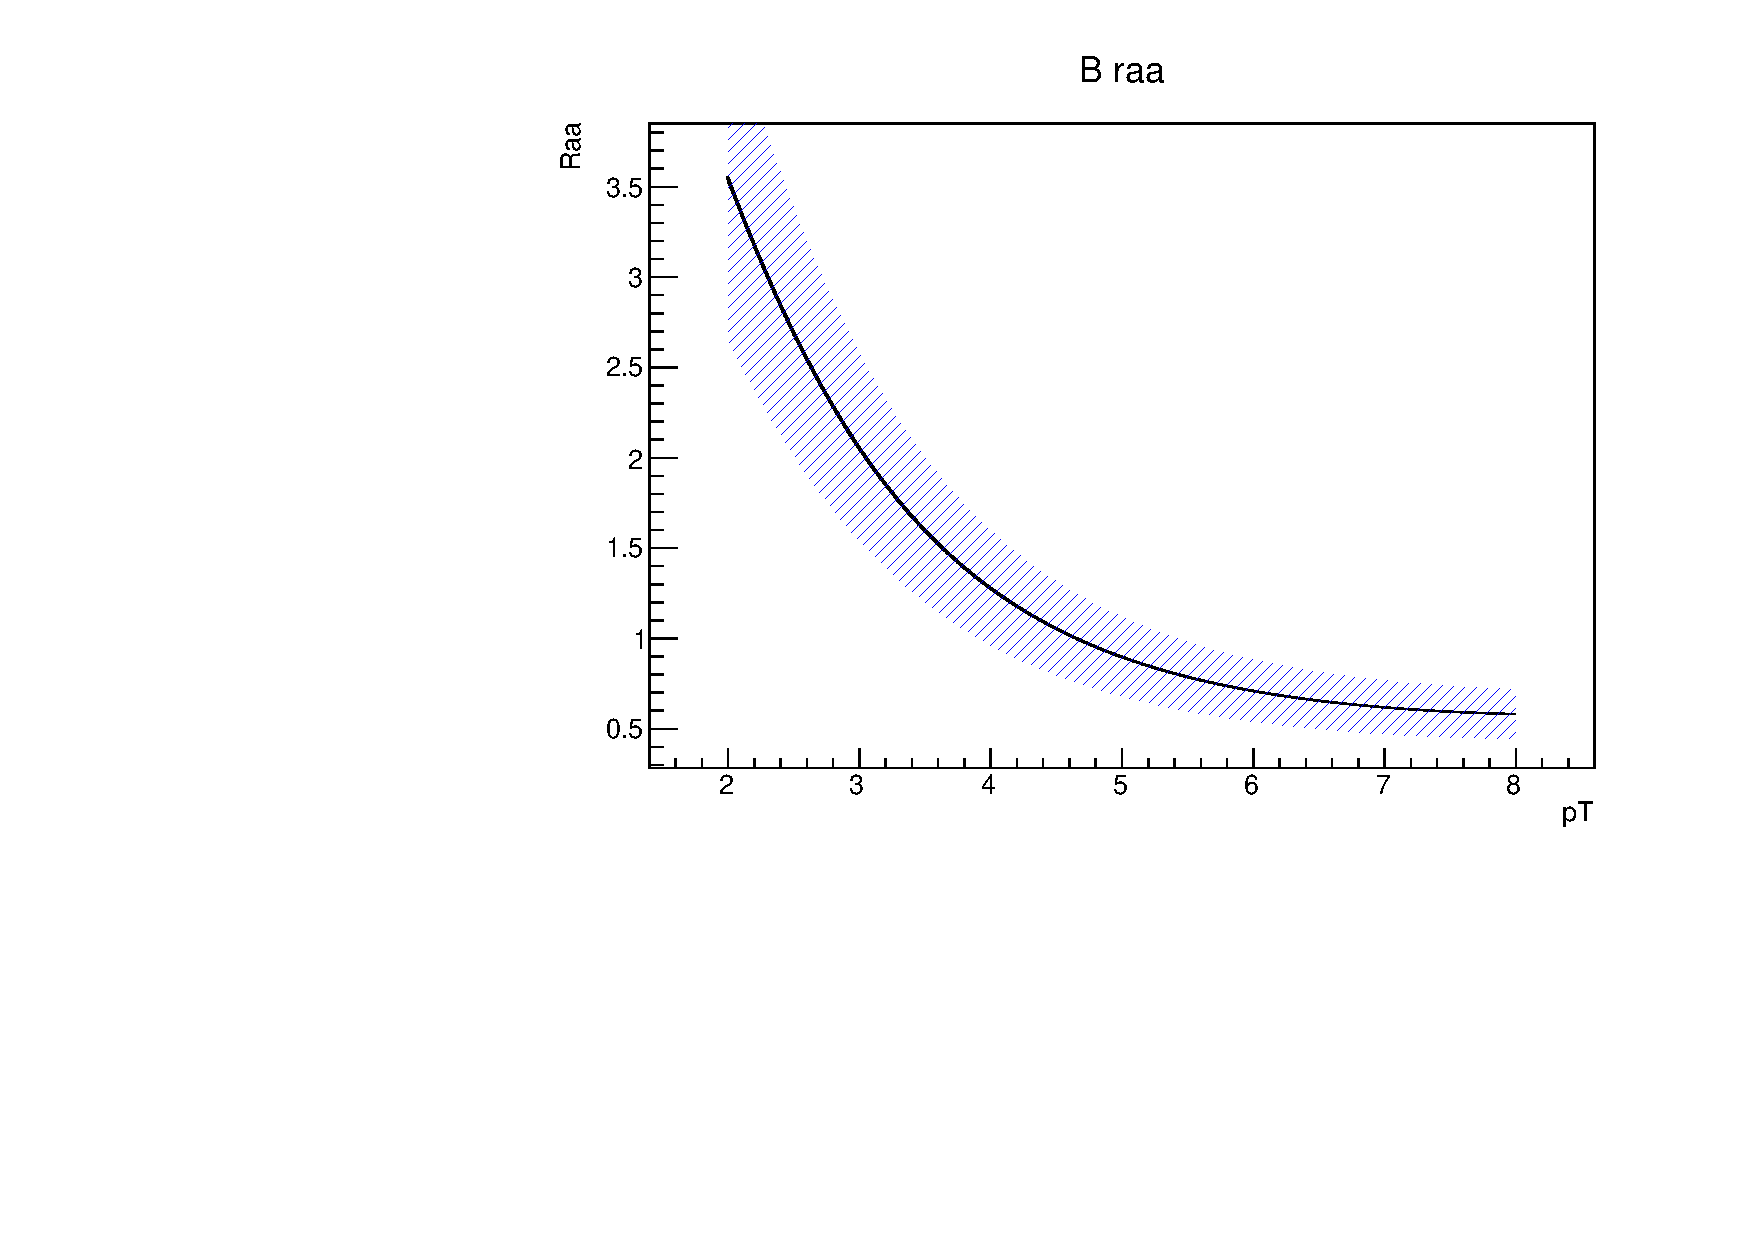
\includegraphics[width=7.5cm]{figures/B.pdf}
	\caption{B介子$R_{AA}$}
	\label{b2b}
\end{subfigure}
\caption{$R_{AA}$的计算结果}
\end{figure}
保留两种pp参考的参数计算出的$R_{AA}$,计算结果如\cref{b2e0,b2d,b2j,b2b}。在误差范围内,Monte Carlo模拟的数据与STAR实验数据 B$\to$e, B$\to$D, B$\to$J/$\psi$ RAA可由同一母粒子分布衰变分析得到,基本验证了数据的可靠性,虽然与B$\to$J/$\psi$分布有一定的偏离。但是,这主要是因为实验处理时B$\to$J/$\psi$ $R_{AA}$的pp参考采用的是与\texttt{FONLL}上限相当的测量结果,导致数据偏低。我们还发现,无论是实验数据还是Monte Carlo数据,pp参考的较大不确定度将导致$R_{AA}$的不确定度较大,说明为提高计算$R_{AA}$的精度,pp参考需要更准确的数据。\par
得到了AA碰撞和pp碰撞B介子谱,我们还首次计算了B的$R_{AA}$。利用定义\cref{raa}将两个L\'evy函数相除,\cref{b2b}可以看到,其在所研究的范围内单调递减,符合夸克在QGP内存在能损的基本结论。

% subsection 结论 (end)

% section 核修正因子 (end)
\newpage
\section{结论} % (fold)
\label{sec:结论}

\begin{enumerate}

	

	\item 在RHIC能区因底夸克产率极低,强子道衰变分支比都在千分之一左右,导致目前为止都没有直接观测的实验结果,我们的工作从已有的实验数据中分析,通过衰变产物产生谱及底强子的衰变运动学,首次提取了底强子的横动量谱。
	\item 我们通过数据驱动(Data Driven)和衰变运动学,提取了底介子的核修正因子$R_{AA}$,实现了首次测量,并给出底夸克在重离子中的产生截面为$\SI{2.16}{\micro\barn}$。
    \item 通过底强子谱的衰变产物分析,我们计算了底强子衰变产物的$R_{AA}$,且在误差范围内与RHIC-STAR观测的实验数据一致。
    \item 我们的得到的结果仍然存在一些误差,其原因可归结为AA实验数据的误差和计算$R_{AA}$时,分母pp碰撞的参考的误差。
\end{enumerate}

% section 结论 (end)

\section{下一步工作展望} % (fold)
\label{sec:下一步工作展望}
下一步将对B介子的$R_{AA}$以及底夸克在AA里的产生截面进行理论分析,与其他粒子的$R_{AA}$进行比较,得到关于重夸克在QGP中演化的物理结论。

我们发现,$R_{AA}$的pp参考部分对整个计算过程的误差贡献最大\cite{Aidala:2019hib}。为了进一步减小误差,我们期望,能够通过更多实验或者通过更精确的QCD微扰理论的算法减小pp参考($R_{AA}$分母分布)不确定度,使得其更加准确。除此以外,不同衰变道低横动量区域测量值的误差均较大,为能够更好地拟合数据,下一步实验工作期望提升该能区的分辨率。

% section 下一步工作展望 (end)


\section{致谢} % (fold)
\label{sec:致谢}

首先感谢张一飞教授提供的研究思路和对本次大研工作总体的指导。其次,感谢司凡学长、陈小龙博士提供的帮助和提供的具体数据。最后,感谢杨承熹同学对笔者安装,调试实用统计软件\texttt{ROOT}及Monte Carlo模拟软件\texttt{PYTHIA8}\cite{Sj_strand_2015}的帮助。

% section 致谢 (end)

% \afterpage{\blankpage}
\bibliographystyle{unsrt}
\bibliography{report}

% \section{\texorpdfstring{$\chi^2$}{chi}检验的说明} % (fold)
% \label{sec:chi方检验的说明}

% 对于假设检验问题$H_0:X$满足分布$f(x)\leftrightarrow H_1:X$不满足分布$f(x)$。已观察到该随机变量的取值-频数,设总频数为$N$。把定义域$[a,b]$分成区间$[a,b]=\bigcup_i [x_i,x_{i+1}]$,在每个区间内,$X$出现的概率应为$\int_{x_i}^{x_{i+1}}f(x)\rd x$。
% \begin{table}[h]\centering
% \begin{tabular}{c|cccc}

% 	\toprule
% 	$X$取值(落在区间内) & $[x_1,x_2]$ & $[x_2,x_3]$& $\cdots$ & $[x_{n},x_{n+1}]$\\
%     观察到的频数$o$ & $n_1$ & $n_2$ & $\cdots$ & $n_{n}$\\
%     期望的频数$e$ &$Np_1$ & $Np_2$ & $\cdots$ &$ Np_n$\\

% 	\bottomrule
% \end{tabular}
% \end{table}

% 按照Pearson-$\chi^2$检验,统计量
% \begin{equation}
% 	x^2 = \sum \frac{(o-e)^2}{e} = \sum_i\frac{\pare{o([x_i,x_{i+1}])-\int_{x_i}^{x_{i+1}}f(x)\rd x}^2}{\int_{x_i}^{x_{i+1}}f(x)\rd x} = \sum_{i=1}^N\frac{f_\text{cal}-f_\text{exp}}{}
% \end{equation}


% section chi方检验的说明 (end)

\end{document} 
